\documentclass{article}

\usepackage{fancyhdr}
\usepackage{extramarks}
\usepackage{amsmath}
\usepackage{amsthm}
\usepackage{amsfonts}
\usepackage{amssymb}
\usepackage{xparse}
\usepackage{tikz}
\usepackage{graphicx}
\usepackage[plain]{algorithm}
\usepackage{algpseudocode}
\usepackage{listings}
\usepackage{hyperref}
\usepackage[per-mode = fraction]{siunitx}
\usepackage{calc}

\usetikzlibrary{automata,positioning}

\hypersetup{
    colorlinks=true,
    linkcolor=blue,
    filecolor=magenta,
    urlcolor=blue,
    }

\urlstyle{same}

%
% Basic Document Settings
%

\topmargin=-0.45in
\evensidemargin=0in
\oddsidemargin=0in
\textwidth=6.5in
\textheight=9.0in
\headsep=0.25in

\linespread{1.1}

\pagestyle{fancy}
\lhead{\hmwkAuthorName}
\chead{\hmwkClass\ (\hmwkClassInstructor,\ \hmwkClassTime): \hmwkTitle}
\rhead{\firstxmark}
\lfoot{\lastxmark}
\cfoot{\thepage}

\renewcommand\headrulewidth{0.4pt}
\renewcommand\footrulewidth{0.4pt}

\setlength\parindent{0pt}
\allowdisplaybreaks
%
% Title Page
%

\title{
	\vspace{2in}
	\textmd{\textbf{\hmwkClass:\ \hmwkTitle}}\\
	\normalsize\vspace{0.1in}\small{Due\ on\ \hmwkDueDate\ at \hmwkDueTime}\\
	\vspace{0.1in}\large{\textit{\hmwkClassInstructor,\ \hmwkClassTime}}
	\vspace{3in}
}
\author{\textbf{\hmwkAuthorName}}
\date{\hmwkCompletionDate}

%
% Create Problem Sections
%

\newcommand{\enterProblemHeader}[1]{
	\nobreak\extramarks{}{Problem #1 continued on next page\ldots}\nobreak{}
	\nobreak\extramarks{Problem #1 (continued)}{Problem #1 continued on next page\ldots}\nobreak{}
}

\newcommand{\exitProblemHeader}[1]{
	\nobreak\extramarks{Problem #1 (continued)}{Problem #1 continued on next page\ldots}\nobreak{}
	\nobreak\extramarks{Problem #1}{}\nobreak{}
}

%
% Homework Problem Environment
%
\NewDocumentEnvironment{hwkProblem}{m m s}{
	\section*{Problem #1: #2}
	\enterProblemHeader{#1}
	\setcounter{partCounter}{1}
}{
	\exitProblemHeader{#1}
	\IfBooleanF{#3} % if star, no new page
		{\newpage}
}

% Alias for the Solution section header
\newcommand{\hwkSol}{\vspace{\baselineskip / 2}\textbf{\Large Solution}\vspace{\baselineskip / 2}}

% Alias for the Solution Part subsection header
\newcounter{partCounter}
\newcommand{\hwkPart}{
	\vspace{\baselineskip / 2}
	\textbf{\large Part \Alph{partCounter}}
	\vspace{\baselineskip / 2}
	\stepcounter{partCounter}
}

%
% Various Helper Commands
%

% Such That
\newcommand{\st}{\text{s.t.}}

% Useful for algorithms
\newcommand{\alg}[1]{\textsc{\bfseries \footnotesize #1}}

% For derivatives
\newcommand{\deriv}[1]{\frac{\mathrm{d}}{\mathrm{d}x} (#1)}

% For partial derivatives
\newcommand{\pderiv}[2]{\frac{\partial}{\partial #1} (#2)}

% Integral dx
\newcommand{\dx}{\mathrm{d}x}
\newcommand{\dy}{\mathrm{d}y}

% Probability commands: Expectation, Variance, Covariance, Bias
\newcommand{\e}[1]{\mathrm{e}#1}
\newcommand{\E}{\mathrm{E}}
\newcommand{\Var}{\mathrm{Var}}
\newcommand{\Cov}{\mathrm{Cov}}
\newcommand{\Bias}{\mathrm{Bias}}

% Defining Units that are not in the SI base
\DeclareSIUnit\bar{bar}
\DeclareSIUnit\ft{ft}
\DeclareSIUnit\dollar{\$}
\DeclareSIUnit\cent{\text{\textcent}}
\DeclareSIUnit\c{\degreeCelsius}

% Code Listing config
\usepackage{xcolor}
\definecolor{codegreen}{rgb}{0,0.6,0}
\definecolor{codegray}{rgb}{0.5,0.5,0.5}
\definecolor{codepurple}{rgb}{0.58,0,0.82}
\definecolor{backcolour}{rgb}{0.95,0.95,0.92}
\lstdefinestyle{overleaf}{
	% backgroundcolor=\color{backcolour},
	commentstyle=\color{codegreen},
	keywordstyle=\color{magenta},
	numberstyle=\tiny\color{codegray},
	stringstyle=\color{codepurple},
	basicstyle=\ttfamily\footnotesize,
	breakatwhitespace=false,
	breaklines=true,
	captionpos=b,
	keepspaces=true,
	numbers=left,
	numbersep=5pt,
	showspaces=false,
	showstringspaces=false,
	showtabs=false,
	tabsize=4
}

\usepackage[latte]{catppuccinpalette}
\lstdefinestyle{catppuccin}{
	breaklines=true,
	keepspaces=true,
	numbers=left,
	numbersep=5pt,
	showspaces=false,
	showstringspaces=false,
	breakatwhitespace=true,
	tabsize=4,
	stringstyle = {\color{CtpGreen}},
	commentstyle={\color{CtpOverlay1}},
	basicstyle = {\small\color{CtpText}\ttfamily},
	keywordstyle = {\color{CtpMauve}},
	keywordstyle = [2]{\color{CtpBlue}},
	keywordstyle = [3]{\color{CtpYellow}},
	keywordstyle = [4]{\color{CtpLavender}},
	keywordstyle = [5]{\color{CtpPeach}},
	keywordstyle = [6]{\color{CtpTeal}}
}

\lstset{style=catppuccin}


%
% Homework Details
%   - Title
%   - Subtitle
%   - Due date
%   - Due time
%   - Course
%   - Section/Time
%   - Instructor
%   - Author
%

\newcommand{\hmwkTitle}{HW 06}
\newcommand{\hmwkSubTitle}{Assignment 6}
\newcommand{\hmwkDueDate}{March 13th, 2025}
\newcommand{\hmwkDueTime}{11:59 PM}
\newcommand{\hmwkClass}{PHYS 313}
\newcommand{\hmwkClassTime}{0101}
\newcommand{\hmwkClassInstructor}{Dr.\ Ji}
\newcommand{\hmwkAuthorName}{\textbf{Vai Srivastava}}
\newcommand{\hmwkCompletionDate}{\today}

\begin{document}

\maketitle

\pagebreak

\begin{hwkProblem}{3.2}{}

	In one sentence, justify Earnshaw's Theorem.

	\hwkSol{}

	Earnshaw's Theorem is justified because in regions free of charges, the electrostatic potential must satisfy Laplace's equation, which prohibits any local minimum or maximum, thereby ensuring that any static configuration of charges is unstable.

\end{hwkProblem}
\begin{hwkProblem}{3.3}{}

	Find the general solution to Laplace's equation in spherical coordinates, for the case where \( V \) depends only on \( r \). Do the same for cylindrical coordinates, assuming \( V \) depends only on \( s \).

	\hwkSol{}

	\hwkPart{}

	\begin{align*}
		\frac{1}{r^{2}}\deriv{r}{r^{2}\deriv{r}{V}} &= 0 \\
		r^{2}\deriv{r}{V} &= C_{1}, \\
		\func{V}[r] &= \frac{C_{1}}{r} + C_{2} \qed
	\end{align*}

	\hwkPart{}

	\begin{align*}
		\frac{1}{s}\deriv{s}{s\deriv{s}{V}} &= 0 \\
		s\deriv{s}{V} &= C_{3}, \\
		\func{V}[s] &= C_{3} \log{s} + C_{4} \qed
	\end{align*}

\end{hwkProblem}
\begin{hwkProblem}{3.4}{}

	\begin{enumerate}
		\item Show that the average electric field over a spherical surface, due to charges outside the sphere, is the same as the field at the center.
		\item What is the average due to charges inside the sphere?
	\end{enumerate}

	\hwkSol{}

	\hwkPart{}

	\begin{align*}
		\nabla^2 \phi &= 0 \\
		\func{\phi}[\vecb{0}] &= \frac{1}{4\pi R^2} \int_{S_R} \func{\phi}[\vecb{r}] \mathrm{d}A \\
		\func{\vecb{E}}[\vecb{r}] &= -\nabla \func{\phi}[\vecb{r}] \\
		\pderiv{x}{\func{\phi}[\vecb{0}]} &=\frac{1}{4\pi R^2}\int_{S_R} \pderiv{x}{\func{\phi}[\vecb{r}]} \mathrm{d}A \\
		\func{E_{x}}[\vecb{0}] &= \frac{1}{4\pi R^2}\int_{S_R} \func{E_{x}}[\vecb{r}] \mathrm{d}A \\
		\langle \vecb{E} \rangle &\equiv \frac{1}{4\pi R^2} \int_{S_R} \func{\vecb{E}}[\vecb{r}] \mathrm{d}A \\
		\langle \vecb{E} \rangle_{\mathrm{ext}} &= \func{\vecb{E}}[\vecb{0}] \qed
	\end{align*}
	Thus, the average field over the sphere (due only to external charges) equals the field at the center.

	\hwkPart{}

	\begin{align*}
	\func{\phi}[\vecb{r}] &= \frac{1}{4\pi \epsilon_0} \left( \frac{Q}{r} + \frac{\vec{p}\cdot\vec{r}}{r^3} + \cdots \right) \\
	Q &= \sum_i q_i \quad \text{and} \quad \vecb{p} = \sum_i q_i\,\vecb{r}_i \\
	\func{\phi_{\text{mon}}}[r] &= \frac{Q}{4\pi\epsilon_0}\frac{1}{r} \\
	\func{\vecb{E}_{\text{mon}}}[r] &= -\nabla \phi_{\text{mon}} = \frac{Q}{4\pi\epsilon_0}\frac{\hat{r}}{r^2} \\
	\langle \hat{r} \rangle &= \frac{1}{4\pi}\int \hat{r}\,d\Omega = \vecb{0} \\
	\func{\phi_{\text{dip}}}[\vecb{r}] &= \frac{1}{4\pi\epsilon_0}\frac{\vecb{p}\cdot\vecb{r}}{r^3} \\
	\func{\vecb{E}_{\text{dip}}}[\vecb{r}] &= -\nabla{\func{\phi_{\text{dip}}}[\vecb{r}]} \\
	\langle \vecb{E} \rangle_{\mathrm{int}} &= -\frac{\vecb{p}}{3\epsilon_0} \qed \\
	\langle r_i r_j \rangle &= \frac{r^2}{3}\delta_{ij} \qed
	\end{align*}
	By integration over the spherical surface, the net average is proportional to \(\vecb{p}\) with the constant of proportionality \(\frac{-1}{3\epsilon_0}\).

\end{hwkProblem}
\begin{hwkProblem}{3.7}{}

	Find the force on the charge \( +q \) in the below image, noting that the \( xy \) plane is a grounded conductor.
	\begin{figure}[H]
		\begin{center}
			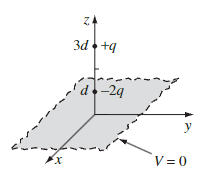
\includegraphics[width=0.35\textwidth]{./images/p3_7.png}
		\end{center}
		\caption{Diagram for Problem 3.7}\label{fig:p3_7}
	\end{figure}

	\hwkSol{}
	
	The net force on the real \(+q\) is given by the Coulomb forces due to the other charges. Since all charges lie on the \(z\)–axis, the force on \(+q\) will be directed along the \(z\)–axis.

	\textbf{1. Force due to the real charge \(-2q\) at \(z=d\):}  

	\[
	r_{1} = 3d - d = 2d.
	\]
	\[
	F_{1} = \frac{1}{4\pi\epsilon_0}\frac{q\,(2q)}{(2d)^2} = \frac{1}{4\pi\epsilon_0}\frac{2q^2}{4d^2} = \frac{q^2}{8\pi\epsilon_0 d^2}.
	\]
	\[
	\mathbf{F}_1 = -\frac{q^2}{8\pi\epsilon_0 d^2}\,\hat{z}.
	\]

	\textbf{2. Force due to the image of \(+q\), namely \(-q\) at \(z=-3d\):}  

	\[
	r_{2} = 3d - (-3d) = 6d.
	\]
	\[
	F_{2} = \frac{1}{4\pi\epsilon_0}\frac{q\,(q)}{(6d)^2} = \frac{q^2}{4\pi\epsilon_0\,(36d^2)} = \frac{q^2}{144\pi\epsilon_0 d^2}.
	\]
	\[
	\mathbf{F}_2 = -\frac{q^2}{144\pi\epsilon_0 d^2}\,\hat{z}.
	\]

	\textbf{3. Force due to the image of \(-2q\), namely \(+2q\) at \(z=-d\):}  

	\[
	r_{3} = 3d - (-d) = 4d.
	\]
	\[
	F_{3} = \frac{1}{4\pi\epsilon_0}\frac{q\,(2q)}{(4d)^2} = \frac{2q^2}{4\pi\epsilon_0\,(16d^2)} = \frac{q^2}{32\pi\epsilon_0 d^2}.
	\]
	Since both charges are positive, the force is repulsive. The vector from the image charge at \(z=-d\) to the real \(+q\) at \(z=3d\) points upward; thus, the force on \(+q\) is upward:
	\[
	\mathbf{F}_3 = +\frac{q^2}{32\pi\epsilon_0 d^2}\,\hat{z}.
	\]

	\textbf{Net Force:}  

	Summing the three contributions we have
	\[
	\mathbf{F} = \mathbf{F}_1 + \mathbf{F}_2 + \mathbf{F}_3 = \left[-\frac{q^2}{8\pi\epsilon_0 d^2} - \frac{q^2}{144\pi\epsilon_0 d^2} + \frac{q^2}{32\pi\epsilon_0 d^2}\right]\hat{z}.
	\]
	\[
	\frac{1}{8} = \frac{18}{144}, \quad \frac{1}{32} = \frac{4.5}{144}.
	\]
	Thus,
	\[
	-\frac{q^2}{8\pi\epsilon_0 d^2} = -\frac{18q^2}{144\pi\epsilon_0 d^2}, \quad
	-\frac{q^2}{144\pi\epsilon_0 d^2} = -\frac{q^2}{144\pi\epsilon_0 d^2}, \quad
	\frac{q^2}{32\pi\epsilon_0 d^2} = \frac{4.5q^2}{144\pi\epsilon_0 d^2}.
	\]
	\[
	\mathbf{F} = -\frac{18q^2}{144\pi\epsilon_0 d^2}\,\hat{z} - \frac{q^2}{144\pi\epsilon_0 d^2}\,\hat{z} + \frac{4.5q^2}{144\pi\epsilon_0 d^2}\,\hat{z} = -\frac{(18+1-4.5)q^2}{144\pi\epsilon_0 d^2}\,\hat{z}.
	\]
	\[
	\mathbf{F} = -\frac{(19 - 4.5)q^2}{144\pi\epsilon_0 d^2}\,\hat{z} = -\frac{14.5\,q^2}{144\pi\epsilon_0 d^2}\,\hat{z}.
	\]
	\[
	\mathbf{F} = -\frac{29\,q^2}{288\pi\epsilon_0 d^2}\,\hat{z} \qed
	\]

	which indicates that the net force on the charge \(+q\) is directed downward (toward the \(xy\)–plane).

\end{hwkProblem}
\begin{hwkProblem}{3.8}{}

	\begin{enumerate}
		\item Using the law of consines, show that the following equations are equivalent:
			\begin{align}
				\func{V}[\vecb{r}] &= \frac{1}{4 \pi \epsilon_{0}} \left( \frac{q}{\rcurs} + \frac{q'}{\rcurs '} \right) \\
				\func{V}[r, \theta] &= \frac{1}{4 \pi \epsilon_{0}} \left[ \frac{q}{\sqrt{r^{2}+a^{2}-2ra\cos\left(\theta\right)}} - \frac{q}{\sqrt{R^{2}+{\left(\frac{ra}{R}\right)}^{2}-2ra\cos\left(\theta\right)}} \right]
			\end{align}
			Where \( r \) and \( \theta \) are the usual spherical polar coordinates, with the \( z \) axis along the line through \( q \). In this form, it is obvious that \( V = 0 \) on the sphere \( r = R \).
		\item Find the induced surface charge on the sphere, as a function of \( \theta \). Integrate this to get the total induced charge. (What \textit{should} it be?)
		\item Calculate the energy of this configuration.
	\end{enumerate}

	\hwkSol{}

	\hwkPart{}

	\begin{align*}
		\func{V}[\vecb{r}]&=\frac{1}{4\pi\epsilon_0}\left(\frac{q}{\left|\vecb{r}-\vecb{r}_q\right|}+\frac{q'}{\left|\vecb{r}-\vecb{r}_{q'}\right|}\right) \\
		\left|\vecb{r}-\vecb{r}_q\right|&=\sqrt{r^2+a^2-2ra\cos\theta} \\
		\vecb{r}_{q'}&=\frac{R^2}{a}\,\hat{z}\quad\text{with}\quad q'=-\frac{qR}{a} \\
		\left|\vecb{r}-\vecb{r}_{q'}\right|&=\sqrt{r^2+\left(\frac{R^2}{a}\right)^2-2r\frac{R^2}{a}\cos\theta} \\
		\func{V}[r, \theta]&=\frac{1}{4\pi\epsilon_0}\left[\frac{q}{\sqrt{r^2+a^2-2ra\cos\theta}}-\frac{q}{\sqrt{R^2+\left(\frac{ra}{R}\right)^2-2ra\cos\theta}}\right]
	\end{align*}
	In this form, when \(r=R\), the two terms cancel (since the geometry is chosen so that the potential on the sphere vanishes), proving the two expressions are equivalent.

	\hwkPart{}

	\begin{align*}
		\func{\sigma}[\theta]&=-\epsilon_0\left.\pderiv{r}{V}\right|_{r=R} \\
		\func{\sigma}[\theta]&=-\frac{q}{4\pi R^2}\,\frac{R^2-a^2}{{\left(R-a\cos{\theta}\right)}^3} \\
		Q_{\text{ind}}&=\int_0^{2\pi}\int_0^{\pi}\func{\sigma}[\theta]\,R^2\sin{\theta}\,\mathrm{d}\theta\,\mathrm{d}\phi \\
		Q_{\text{ind}}&=-q \qed
	\end{align*}

	\hwkPart{}

	\begin{align*}
		U&=\frac{1}{2}\,\frac{q\,q'}{4\pi\epsilon_0}\,\frac{1}{\left|a-\frac{R^2}{a}\right|} \\
		\left|a-\frac{R^2}{a}\right|&=\frac{a^2-R^2}{a} \\
		U&=-\frac{q^2R}{8\pi\epsilon_0}\,\frac{1}{a^2-R^2} \qed
	\end{align*}

\end{hwkProblem}
\begin{hwkProblem}{3.13}{}
	
	Find the potential in the infinite slot of Ex3.3 if the boundary at \( x = 0 \) consists of two metal strips: one, from \( y = 0 \) to \( y = \frac{a}{2} \), is held at a constant potential \( V_{0} \), and the other, from \( y = \frac{a}{2} \) to \( y = a \), is at potential \( -V_{0} \).

	\hwkSol{}

	Similar to the answer in Ex3.3, the configuration retains its independence from \( z \). We again have to solve Laplace's equation but subjected to different boundary conditions:
	\[
		\pderivsec{x}{V} + \pderivsec{y}{V} = 0,
		\begin{cases}
			V = 0 & y = 0 \\
			V = 0 & y = a \\
			V = V_{0} & 0 < y < \frac{a}{2}, x = 0 \\
			V = -V_{0} & \frac{a}{2} < y < a, x = 0 \\
			V \to 0 & x \to \infty
		\end{cases}
	.\]
	This can be accomplished using a similar technique as Griffiths, as follows:
	\begin{align*}
		Y \derivsec{x}{X} + X \derivsec{y}{Y} &= 0 \\
		\frac{1}{X} \derivsec{x}{X} + \frac{1}{Y} \derivsec{y}{Y} &= 0 \\
		\derivsec{x}{X} = k^{2}X ,& \quad \derivsec{y}{Y} = -k^{2}Y \\
		\func{X}[x] = Ae^{kx}+Be^{-kx} ,& \quad \func{Y}[y] = C \sin{ky} + D \cos{ky} \\
		\func{V}[x, y] &= \left(Ae^{kx}+Be^{-kx}\right) \left(C \sin{ky} + D \cos{ky}\right) \\
		\text{condition (v)} &\implies A = 0 \\
		\therefore \func{V}[x, y] &= e^{-ky} \left(C \sin{ky} + D \cos{ky}\right) \\
		\text{condition (i)} &\implies D = 0 \\
		\therefore \func{V}[x, y] &= C e^{-ky} \sin{ky} \\
		\text{condition (ii)} &\implies \sin{ka} = 0 \\
		\therefore k &= \frac{n\pi}{a}, \quad n = \left\{1, 2, 3, \dots\right\} \\
		\func{V}[x, y] &= \sum_{n=1}^{\infty}C_{n}e^{-n \pi \frac{x}{a}} \sin{n \pi \frac{y}{a}}
	\end{align*}
	Here is where we diverge from Griffiths' Ex3.3. We want to fulfill our conditions (iii) and (iv) as follows:
	\begin{align*}
		\func{V}[0, 0<y<\frac{a}{2}] &= \sum_{n=1}^{\infty}C_{n}e^{-n \pi \frac{x}{a}} \sin{n \pi \frac{y}{a}} = V_{0}, \\
		\func{V}[0, \frac{a}{2}<y<a] &= \sum_{n=1}^{\infty}C_{n}e^{-n \pi \frac{x}{a}} \sin{n \pi \frac{y}{a}} = -V_{0}.
	\end{align*}
	The Fourier sine coefficients are given by:
	\begin{align*}
		C_n &= \frac{2}{a}\int_{0}^{a} \func{f}[y]\sin{n \pi \frac{y}{a}}\mathrm{d}y \\
		C_n &= \frac{2}{a}\left[\int_{0}^{a/2} V_0\,\sin{n \pi \frac{y}{a}}\mathrm{d}y + \int_{a/2}^{a} (-V_0)\,\sin{n \pi \frac{y}{a}}\mathrm{d}y\right] \\
		\int_{0}^{a/2} \sin{n \pi \frac{y}{a}}\mathrm{d}y &= {\left[-\frac{a}{n\pi}\cos{n \pi \frac{y}{a}}\right]}_{0}^{a/2} \\
		&=\frac{a}{n\pi}{\left[1-\cos{\frac{n\pi}{2}}\right]} \\ 
		\int_{a/2}^{a} \sin{\frac{n\pi y}{a}}\mathrm{d}y &= {\left[-\frac{a}{n\pi}\cos{n \pi \frac{y}{a}}\right]}_{a/2}^{a} \\
		&=\frac{a}{n\pi}\left[\cos{\frac{n\pi}{2}}-\cos{n\pi}\right] \\
		C_n &= \frac{2V_0}{n\pi}\left[\left(1-\cos{\frac{n\pi}{2}}\right)-\left(\cos{\frac{n\pi}{2}}-\cos{n\pi}\right)\right] \left(1-\cos{\frac{n\pi}{2}}\right)-\left(\cos{\frac{n\pi}{2}}-\cos{n\pi}\right) \\
		&= 1 -\cos{\frac{n\pi}{2}}-\cos{\frac{n\pi}{2}}+\cos{n\pi} \\
		&= 1 - 2\cos{\frac{n\pi}{2}}+\cos{n\pi}
	\end{align*}
	Thus, the solution becomes:
	\[
		\func{V}[x, y]=\sum_{n\,\text{odd}} \frac{4V_0}{n\pi}\,e^{-n\pi \frac{x}{a}}\sin{n \pi \frac{y}{a}} \qed
	\]

\end{hwkProblem}
\end{document}